\section{Backend}
	V rámci backendové nebo-li serverové části projektu je prvně nutné zmínit, že funguje na principu API - tzn. že na ní přicházejí požadavky od klienta a na ně náležitě odpovídá. Nevrací ani nijak nespravuje vizualizaci dat - jen předává data na frontendovou část, o které je psáno dále.
	
	Zde jsou zobecněné základní úkony, které v mé implementaci právě backend vykonává:
	
	\begin{itemize}
		\item Zpracování a vyřizování požadavků z webové frontendové části
		\item Administraci databáze - tzn. vytváření, úpravu, mazání a čtení jednotlivých objektů a migrace databáze (tj. automatizovaná deklarace struktury databázového objektu)
		\item Rozesílání emailů (např. pozvánky na neveřejný formulář)
		\item Exportování dat do Excel tabulek
		\item Autentifikaci uživatele
	\end{itemize}
	 
	V následující části jsou popsány jednotlivé backendové komponenty a principy, díky kterým je celý projekt implementován.
	
	\subsection{Obecná struktura Laravel projektu}
	Prvně je nutné rozebrat obecnou strukturu Laravel projektu. 
		\begin{figure}[H]
			\centering %% příkaz, který ti obrázek zarovná na střed
			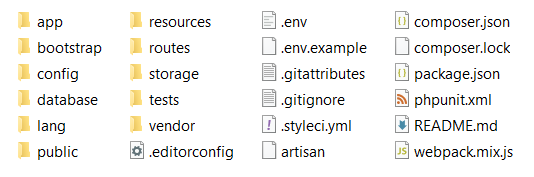
\includegraphics[width=0.9\textwidth]{img/laravel_struktura.png} %% vložení samotného obrátku
			\caption{Obecná struktura nově vygenerovaného Laravel projektu} %% popisek obrázku, nezapomeň na citace!
			\label{fig:laravel_str} %% označení až budeš chtít na obrázek odkazovat
		\end{figure}
	%% obrázek struktury složky
	Jak můžeme na obrázku výše vidět, celý projekt je složen z mnoha složek a souborů. Jelikož podrobný rozbor jednotlivých částí není předmětem této práce, tak jsou nejdůležitější části pro implementaci projektu popsány níže jen obecně.
	\begin{itemize}
		\item Složka \textit{app} obsahuje většinu tříd jádra aplikace
		\item Složka \textit{bootstrap} obsahuje soubory pro zavedení a spuštění aplikace
		\item Složka \textit{config} obsahuje konfigurace jednotlivých částí aplikace
		\item Složka \textit{database} obsahuje soubory spojené s prací s databázi
		\item Složka \textit{lang} obsahuje soubory jazyků a překladů (zde nevyužita)
		\item Složka \textit{public} obsahuje soubory, které jsou veřejně dostupné při uživatelské interakci s aplikací (např. při načtení webu v prohlížeči)
		\item Složka \textit{resources} obsahuje pohledy a nezkompilované soubory pro celý frontend
		\item Složka \textit{routes} obsahuje všechny definice cest aplikace (např. cestu \textit{/api/forms/create} pro vyřízení požadavku vytvoření nového formuláře)
		\item Složka \textit{storage} obsahuje primárně záznamy o chodu aplikace a jiné aplikací vygenerované soubory
		\item Složka \textit{tests} obsahuje automatizované testy aplikace (zde nevyužita)
		\item Složka \textit{vendor} obsahuje závislosti a soubory přídavných balíčků, které aplikace používá 
		\item Soubor .env držící veškeré důležité administrativní hodnoty jako např. přihlašovací údaje k databázi
		\item Soubor artisan obsahující důležité příkazy pro stavbu aplikace \cite{LaravelArtisan}
		\item Soubor composer.json držící informace o přídavných balíčcích pro Laravel projekt \cite{ComposerpJSON}
		\item Soubor package.json držící informace o přídavných balíčcích pro frontendovou část projektu \cite{NPMpJSON}
		\item Soubor webpack.mix.js obsahující informace pro kompilaci souborů pro frontend \cite{LaravelJSCSS}
	\end{itemize} \cite{LaravelDir}

	\subsection{Modely}
	Modely slouží k mapování jednotlivých dat z databáze a jsou zprostředkovány pomocí objektově-relačního mapovacího balíčku Eloquent. Pro správnou funkčnost musí být zajištěno, že má každá tabulka v databázi vlastní model. Díky tomuto přístupu lze s daty manipulovat tak, že vytvoříme instanci příslušné třídy a na ní voláme příslušné metody (např. \textit{update} pro změnu záznamů). *cite https://laravel.com/docs/8.x/eloquent*
	
	V rámci tohoto projektu vzniklo mnoho modelů, které mapují většinu tabulek databáze (v kontextu mnou vytvořených modelů nejsou vytvořeny modely např. pro předgenerované tabulky jako \textit{migrations} nebo \textit{failed\_jobs}). Kromě samotné funkce mapování dat z databáze jim můžeme přiřazovat různé vlastnosti a metody, díky kterým lze měnit např. chování při předávání dat. Nejdůležitější a mnou použité jsou v následujícím seznamu:
	
	\begin{itemize}
		\item Metody vytvářející vazby mezi modely - Ty určují jednotlivé vztahy mezi modely a slouží k jednodušší práci s daty. Existuje mnoho metod - např. belongsTo (označuje, komu samotný model náleží) či hasOne/hasMany (označuje, které model/y samotnému modelu patří).
		\item Vlastnost \textit{fillable} - Ta určuje, do kterých atributů může být na vrstvě webové aplikace zapisováno. Nenapíšeme sem tedy např. \textit{id}, které většinou chceme doplnit až při uložení do databáze samotnou databází.
		\item Vlastnost visible - Ta určuje, které atributy jsou ve vrácených datech z databáze viditelné a tedy poslané dále (myšleno na frontend aplikace). Např. z bezpečnostního hlediska sem nenapíšeme atribut uživatelského hesla, který by neměl být obecně předáván mimo server.
		\item Vlastnost table - Ta slouží k přesnému určení tabulky pomocí jejího jména, ke které se vytvořený model vztahuje.
		\item Vlastnost with - Ta slouží k výchozímu připojení dalších dat z jiného modelu ke stávajícímu setu dat modelu. K takovému úkonu je nutné mít vytvořené vazby pomocí příslušných metod.
	\end{itemize} *cite https://laravel.com/docs/8.x/eloquent*

	Každý model většinou nevyužívá všechny zmíněné činnosti, ale jen ty, které jsou pro jeho typ důležité. Příkladem je zde uveden poměrně rozsáhlý model formuláře \textit{Form}. Podobným způsobem jsou vytvořeny i ostatní modely.
	
	Třída modelu Form reprezentuje jednotlivé formuláře. Odkazuje se na stejnojmennou tabulku \textit{forms}, ze které přebírá data. Má definované vlastnosti: \textit{fillable} (např. jméno formuláře, popis formuláře, čas spuštění, ID uživatele, kterému formulář patří,...), \textit{visible} (např. atributy jako jméno formuláře, odkaz na formulář či popis formuláře, ale také názvy atributů, které jsou přidávány v průběhu práce s daty, a názvy metod vytvářejících vazby mezi některými dalšími modely jako např. pro model uživatele, pro kterého platí, že mu formulář musí náležet) a \textit{with} (zde jen název vazbové metody pro model elementu formuláře, u kterého platí, že musí formuláři náležet a že jednomu formuláři může náležet i více elementů). Samotná definice provázání modelu s tabulkou v databázi pomocí vlastnosti table zde není potřeba - Laravel umí u jednoduše pojmenovaných modelů vygenerovaných pomocí Artisan skriptů tuto vlastnost vnitřně doplnit.
	
	%%obrázek modelu php
	\begin{figure}[H]
		\begin{figure}[H]
			\centering
			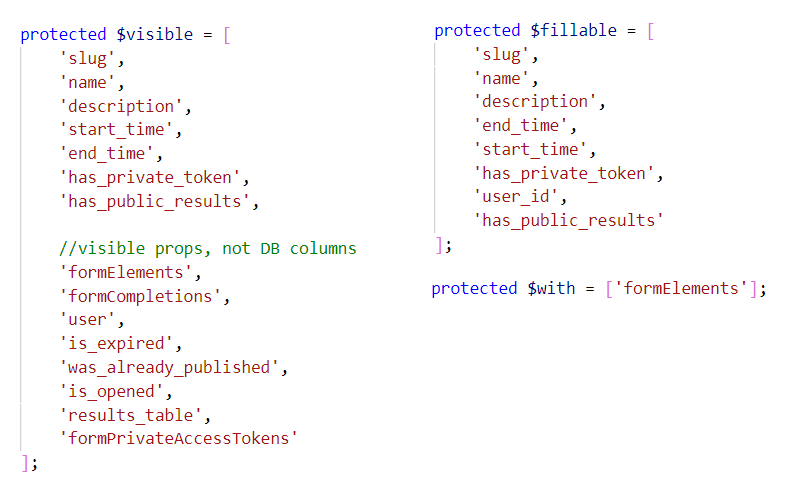
\includegraphics[width=0.8\textwidth]{img/form_model/vlastnosti.png}
			\caption{Zmíněné vlastnosti modelu formuláře}
			\label{fig:model_vlastnosti}
		\end{figure}
		
		\begin{figure}[H]
			\centering
			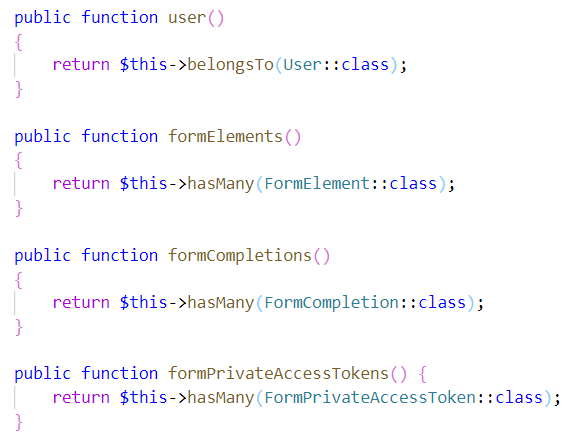
\includegraphics[width=0.7\textwidth]{img/form_model/metody.png}
			\caption{Zmíněné metody modelu formuláře}
			\label{fig:model_metody}
		\end{figure}
	\end{figure}
	
	
	
			
	\subsection{Kontrolery}
	
	
	\subsection{Exporty}
	
	\subsection{Maily}
	
	\subsection{Migrace databáze}
		\subsubsection{Factories}
	
	\subsection{Pohledy}
	
	\subsection{Routes}
	
	\subsection{Průběh jednotlivých činností}
		\subsubsection{Ukládání formuláře}
		\subsubsection{Mazání formuláře}
		%% atd.


